% Options for packages loaded elsewhere
\PassOptionsToPackage{unicode}{hyperref}
\PassOptionsToPackage{hyphens}{url}
%
\documentclass[
  12pt,
]{article}
\usepackage{amsmath,amssymb}
\usepackage{iftex}
\ifPDFTeX
  \usepackage[T1]{fontenc}
  \usepackage[utf8]{inputenc}
  \usepackage{textcomp} % provide euro and other symbols
\else % if luatex or xetex
  \usepackage{unicode-math} % this also loads fontspec
  \defaultfontfeatures{Scale=MatchLowercase}
  \defaultfontfeatures[\rmfamily]{Ligatures=TeX,Scale=1}
\fi
\usepackage{lmodern}
\ifPDFTeX\else
  % xetex/luatex font selection
\fi
% Use upquote if available, for straight quotes in verbatim environments
\IfFileExists{upquote.sty}{\usepackage{upquote}}{}
\IfFileExists{microtype.sty}{% use microtype if available
  \usepackage[]{microtype}
  \UseMicrotypeSet[protrusion]{basicmath} % disable protrusion for tt fonts
}{}
\makeatletter
\@ifundefined{KOMAClassName}{% if non-KOMA class
  \IfFileExists{parskip.sty}{%
    \usepackage{parskip}
  }{% else
    \setlength{\parindent}{0pt}
    \setlength{\parskip}{6pt plus 2pt minus 1pt}}
}{% if KOMA class
  \KOMAoptions{parskip=half}}
\makeatother
\usepackage{xcolor}
\usepackage[margin=1in]{geometry}
\usepackage{graphicx}
\makeatletter
\def\maxwidth{\ifdim\Gin@nat@width>\linewidth\linewidth\else\Gin@nat@width\fi}
\def\maxheight{\ifdim\Gin@nat@height>\textheight\textheight\else\Gin@nat@height\fi}
\makeatother
% Scale images if necessary, so that they will not overflow the page
% margins by default, and it is still possible to overwrite the defaults
% using explicit options in \includegraphics[width, height, ...]{}
\setkeys{Gin}{width=\maxwidth,height=\maxheight,keepaspectratio}
% Set default figure placement to htbp
\makeatletter
\def\fps@figure{htbp}
\makeatother
\setlength{\emergencystretch}{3em} % prevent overfull lines
\providecommand{\tightlist}{%
  \setlength{\itemsep}{0pt}\setlength{\parskip}{0pt}}
\setcounter{secnumdepth}{5}
\usepackage{setspace,lscape} \usepackage{amsmath} \usepackage{array} \usepackage{caption,subcaption} \usepackage{longtable} \usepackage{booktabs} \usepackage{enumitem} \usepackage{standalone} \renewcommand{\arraystretch}{1.5} \captionsetup[table]{skip=5pt} \setstretch{1.5}
\ifLuaTeX
  \usepackage{selnolig}  % disable illegal ligatures
\fi
\usepackage[]{natbib}
\bibliographystyle{apalike}
\IfFileExists{bookmark.sty}{\usepackage{bookmark}}{\usepackage{hyperref}}
\IfFileExists{xurl.sty}{\usepackage{xurl}}{} % add URL line breaks if available
\urlstyle{same}
\hypersetup{
  pdftitle={Experiment Results},
  pdfauthor={Zark Zijian Wang},
  hidelinks,
  pdfcreator={LaTeX via pandoc}}

\title{Experiment Results}
\author{Zark Zijian Wang}
\date{October 22, 2023}

\begin{document}
\maketitle

\hypertarget{survey-desigm}{%
\section{Survey Desigm}\label{survey-desigm}}

We use a within-subjects design. The survey contains 23 choice
questions, of which 20 questions are intertemporal choices and 3
questions are risky choices. Each question consists of a choice list. In
an intertemporal choice question, there are 10 rows in the list. In each
row, participants are required to choose between a single immediate
reward (labelled as ``option A'') and a two-reward sequence, constituted
by an immediate reward and a delayed reward (labelled as ``option B'').
Option A is constant within a question, while option B varies from row
to row. Participants need to actively and explicitly state their
preferences on each choice. The risky choice questions follow a similar
pattern. In each row of a risky choice question, participants can choose
either to get a large reward with a 50\% chance or to get a small reward
with certainty. The risky reward is constant within the question, while
the safe reward varies across rows. We use these risky choice questions
to characterize the participants' utility function for further analysis.

The intertemporal choice questions are presented with a random order.
Two of such questions are used for attention check. In one attention
check question, the immediate reward in the sequence option (option B)
dominates the amount of the single-reward option (option A) in each row;
in another question, the latter dominates the sum of both rewards in
option B. Particpants are presumed to only choose option B for all rows
on the first attention check question, and only choose option A on the
second question.

The remaining intertemporal choice questions are divided into two
conditions: the first condition is called ``\emph{Immediate reward
varies}''; the second condition is called ``\emph{Delayed reward
varies}''. In each question under the ``Immediate reward varies''
condition, the immediate reward in the sequence option increases by £10
with each row, starting from £10 and going up to £100, whereas the
delayed reward in that option remains constant for all rows. In each
question under the ``Delayed reward varies'' condition, the amount of
the delayed reward in the sequence option varies across rows, following
the same pattern as the first condition, while the immediate reward in
that option remains constant. Under each condition, the time length of
the sequence option, e.g.~when the delayed reward is delivered, is also
constant across rows in a choice list.

\begin{figure}
  \vspace{16pt}
  \centering
  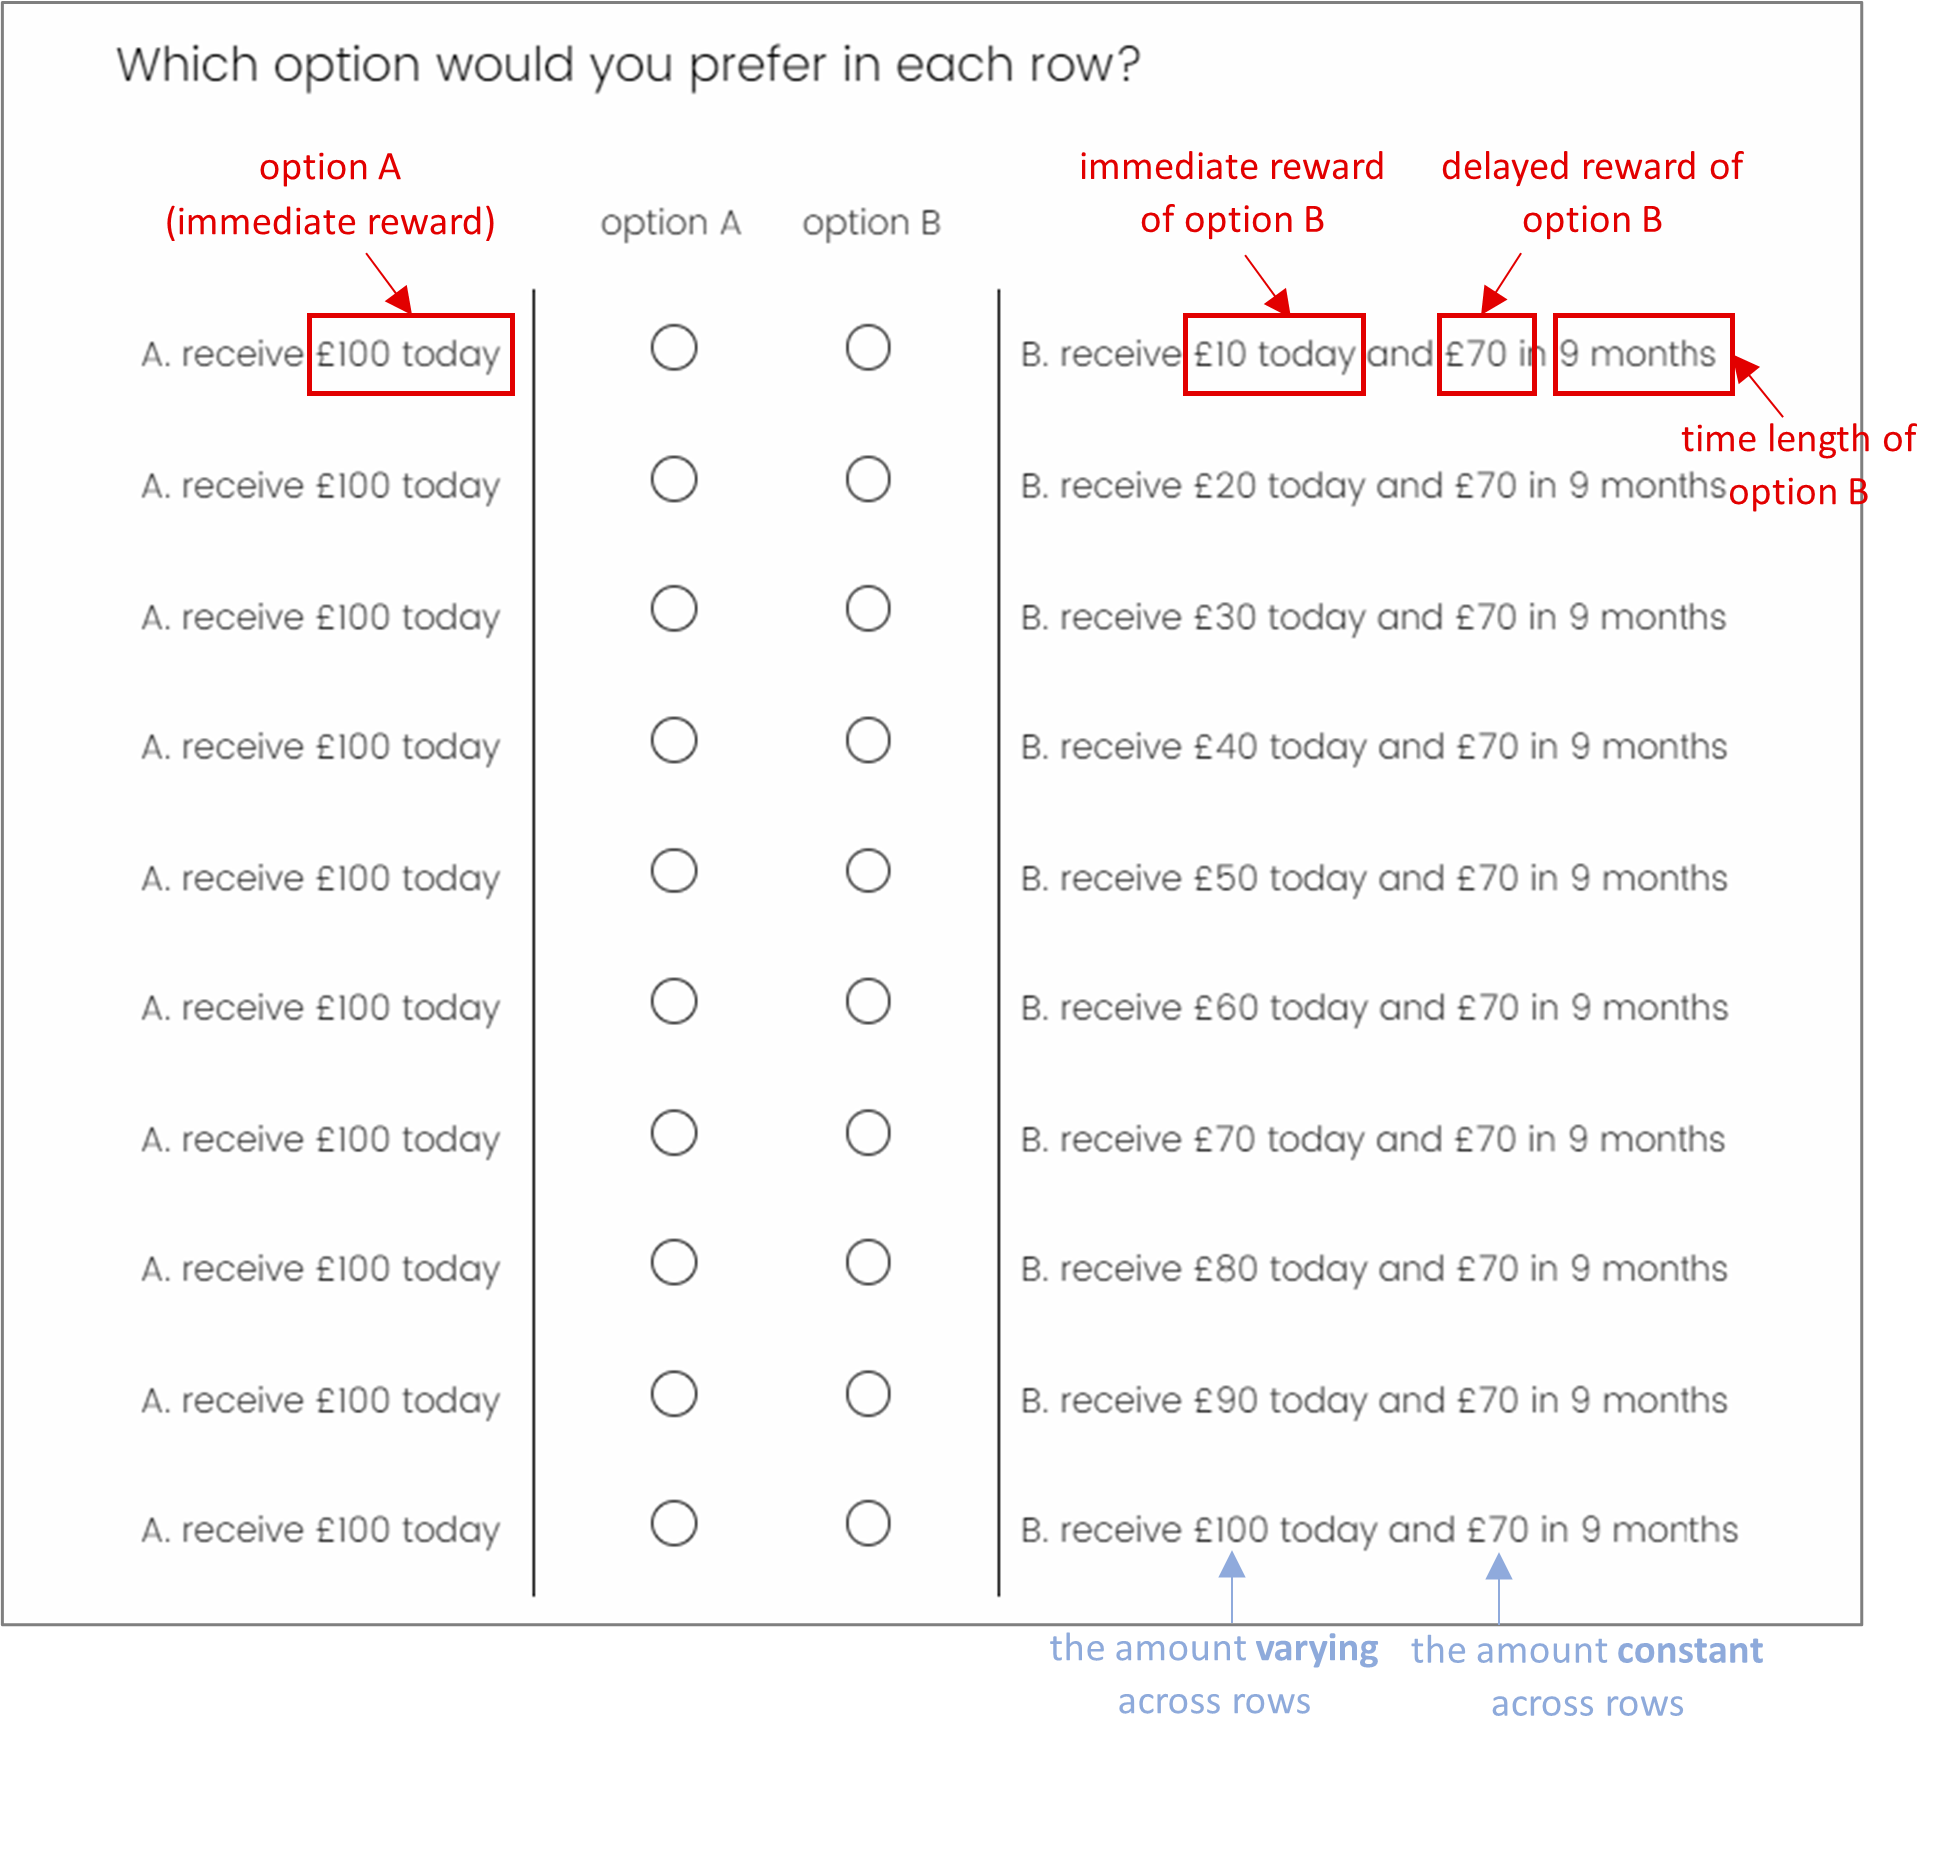
\includegraphics[width=0.96\textwidth]{figures/screenshot.png}
  \caption{Screenshot of an intertemporal choice question}
  \label{fig:question}
\end{figure}

The amount of the single-reward option is selected from \{£100, £120\}.
Each of such amounts is paired with a combination of a
constant-across-rows amount and a time length of the sequence option.
The constant-across-rows amount in any sequence is selected from \{£50,
£70, £90\}. Under the ``Immediate reward varies'' condition, the time
length of a sequence is selected from \{1 month, 9 months, 18 months\}.
The delayed reward is constant within a question, the lowest level of it
is combined with the shortest time length (1 month), the middle level of
it is combined with the shortest or middle time length (1 month or 9
months), and the highest level of it is combined with every level of
time length (1 month, 9 months or 18 months). By this approach, we
obtain 6 combinations and thus \(6\times2=12\) questions (paired with
each amount of the single-reward option) for this condition. Under the
``Delayed reward varies'' condition, we only examine whether the
variation of the immediate reward amount in a sequence will interfere
the impact of the delayed reward amount in choices. So, the time length
is simply set to 3 months. This time length is combined with each level
of the immediate reward amount, which is constant-across-rows under this
condition. Pairing with the amounts for single-reward option, we obtain
\(3\times2=6\) questions for the second condition. Overall, there are 18
intertemporal choice questions for analysis.

\hypertarget{data}{%
\section{Data}\label{data}}

We recruited 160 participants via Prolific. All the participants are
British residents; 50\% of them are female, and the median age is 41. On
average, it took around 11.6 minutes for participants to finish the
survey, with nine tenths of the participants finishing within 20
minutes. Each participants received £2 after completing the survey.
Three participants failed the attention check. We remove these three
participants and remain 157 participants in the sample. Each
participants completed 12 questions under the ``Immediate reward
varies'' condition and 6 questions under the ``Delayed reward varies''
condition. Given that each intertemporal choice question contains 10
rows, we obtain 18,840 observations (choices) for the first condition
and 9,420 observations (choices) for the second condition.

\hypertarget{hypothesis}{%
\section{Hypothesis}\label{hypothesis}}

We developed two hypotheses:

\setlength{\leftskip}{24pt}

(H1) \emph{When a two-reward sequence has a larger reward amount in one
specific period, people's choices are less sensitive to the changes in
the other reward amount.}

(H2) \emph{When a two-reward sequence has a longer time length, people's
choices are less sensitive to the changes in the immediate reward
amount.}

\setlength{\leftskip}{0pt}

For illustration, suppose a set of individuals are required to both
choose between ``receive £100 today'' (option A) and ``receive £50 today
and £70 in 1 month'' (option B1), and choose between option A and
``receive £50 today and £90 in 1 month'' (option B2). Note B2 is the
same as B1 except having a larger delayed reward amount. If the
immediate reward (£50) in option B1 goes up to £60, each individual are
more likely to prefer option B1 over option A. Then, if the immediate
reward in B2 is also raised to £60, our H1 predicts that fewer
individuals will act on this increase, i.e.~shifting from option A to
B2, compared to the responses observed for B1 (since they are ``less
sensitive'' to the given change). Besides, consider a choice between
option A and ``receive £50 today and £70 in 9 months'' (option B3; the
same as B1 except having a longer time length). Our H2 predicts that,
compared to the choices involving B1, for the same increase in the
immediate reward in B3, fewer indiviuals will shift from option A to B3.

We validate our hypotheses by two approaches. First, in a descriptive
analysis, we estimate the indifference point between such option A and
B. A smaller variance in such indifference points among participants
implies a greater sensitivity of choice to the changes in option B. In
an extreme case, suppose in a choice list, every participant prefers
``receive £100 today'' (option A) over ``receive £50 today and £70 in 1
month'' (option B1), but in the next row, they all prefer ``receive £60
today and £70 in 1 month''. Then, every participants' indifference point
is between £50 and £60; they exhibit no variance in their chocies. In
other words, at the point of B1, increasing the immediate reward by £10
leads all participants to shift from option A to option B; at that
point, they are extremely sensitive to the given change.

Second, by logistic regression, we estimate the probability of choosing
option B in each choice. We examine the choice sensitivity by adding
interactions between different elements in option B into independent
variables. For instance, in the ``Immediate reward varies'' condition,
if the regression result suggests, under a time length of 9 months, one
unit increase in the immediate reward of option B, on average yields a
smaller increase in choice probability for option B than that under a
time length of 1 month. Then, we can conclude that people are less
sensitive to the given change under the former time length.

\hypertarget{descriptive-analysis}{%
\section{Descriptive Analysis}\label{descriptive-analysis}}

We estimate the indifference point in varying-across-rows amounts
between the single-reward option (option A) and sequence options (option
B) for each intertemporal choice question. Suppose in a choice list
under the ``Immediate reward varies'' condition, one participant prefers
option A when option B is ``receive £50 today and £70 in 1 month'', but
in the next row, when option B is ``receive £60 today and £70 in 1
month'', she prefers option B. Then, we set £55, i.e.~the median between
£50 and £60, as her indifference point for this question. Figure
\ref{fig:choice-sd} shows the standard deviation of indifference points
among participants for each question.

\begin{figure}
  \centering
  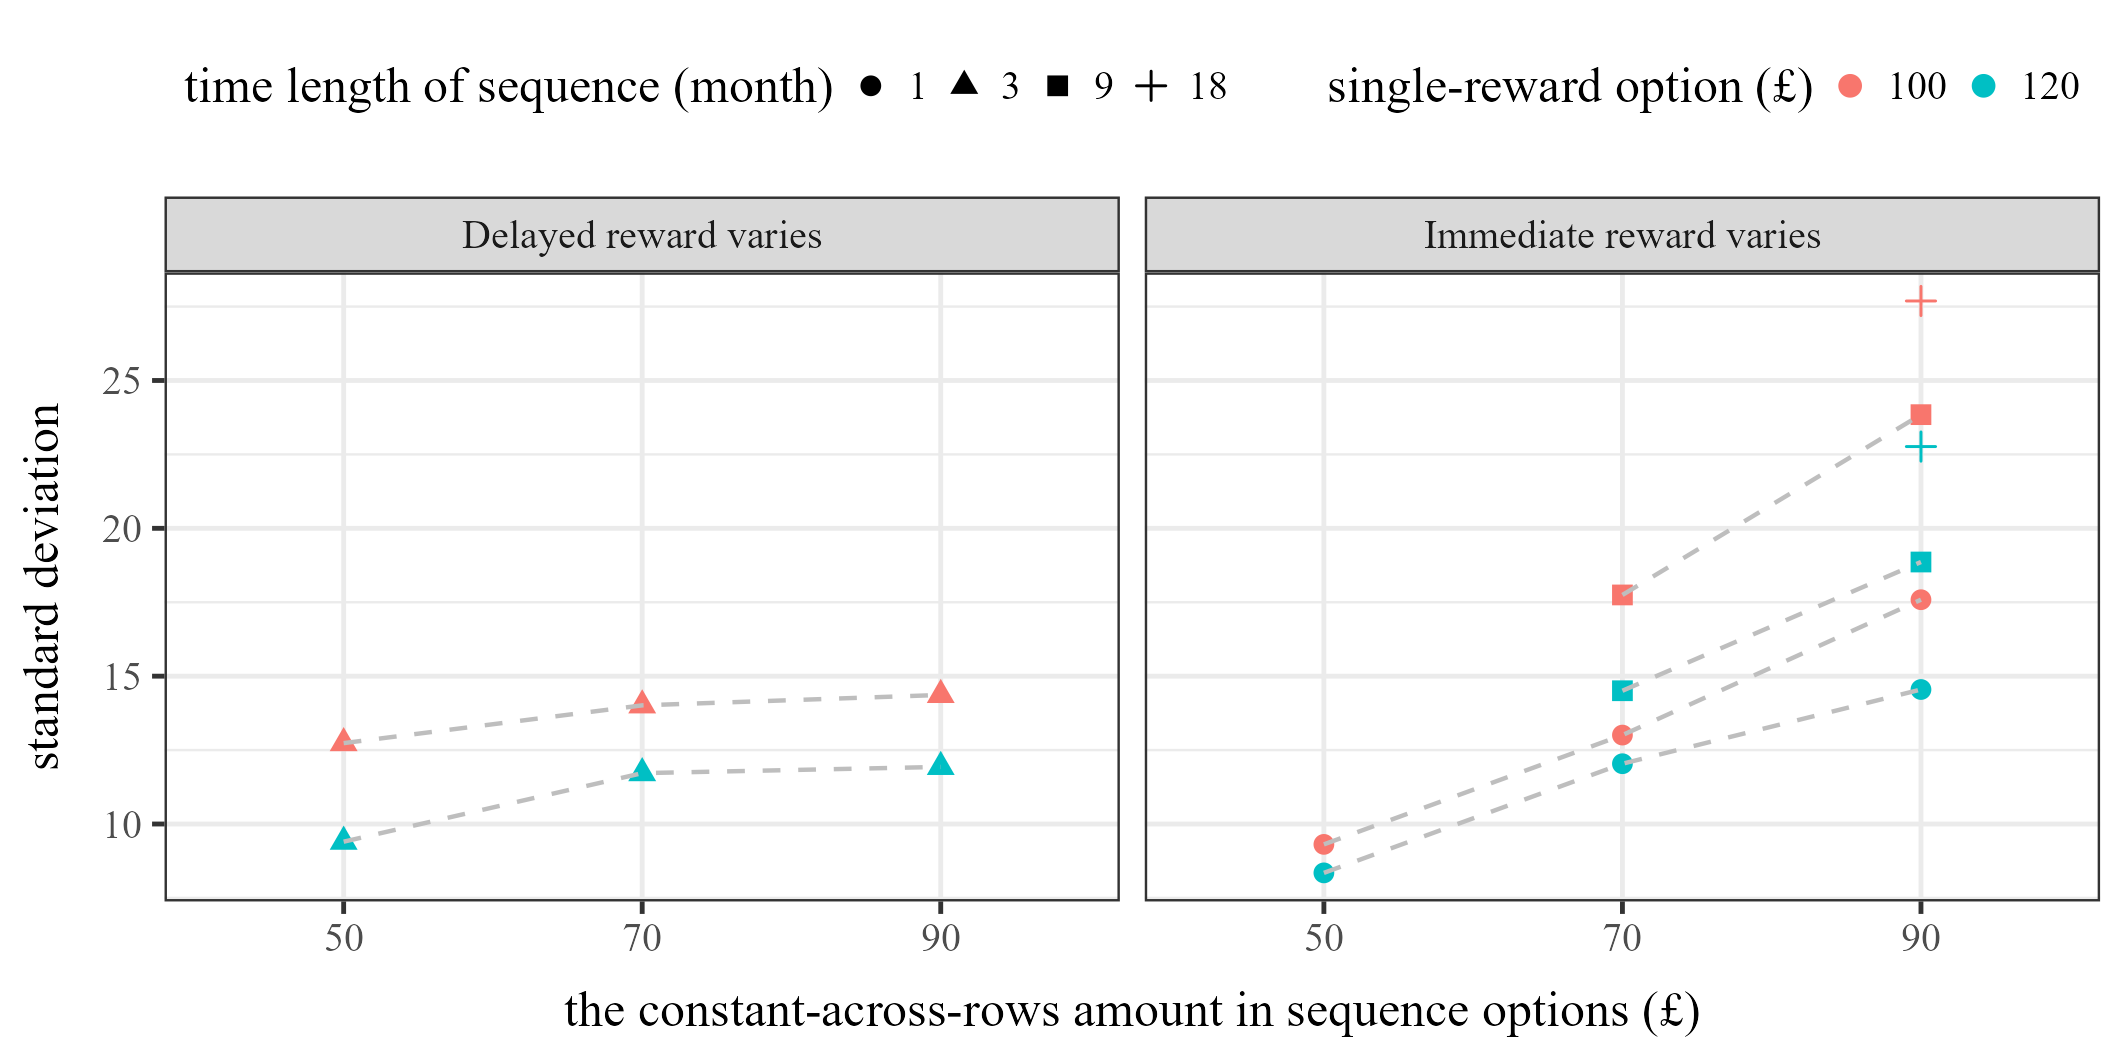
\includegraphics[width=0.96\textwidth]{figures/fig_switch_sd.png}
  \caption{Standard deviation of indifference points in intertemporal choice questions}
  \label{fig:choice-sd}
\end{figure}

Figure \ref{fig:choice-sd} has three notable properties. First, under
each condition, when the constant-across-rows amount in a sequence is
increased (with the others being equal), the standard deviation of
indifference points increases. This is consistent with H1. Second, under
the ``Immediate reward varies'' condition, when the time length of a
sequence is increased, the standard deviation of indifference points
also increases. This is consistent with H2. Finally, under each
condition, when the single-reward option is increased from £100 to £120,
the standard deviation of indifference points increases as well.

\hypertarget{regression-analysis}{%
\section{Regression Analysis}\label{regression-analysis}}

\hypertarget{baseline-model}{%
\subsection{Baseline Model}\label{baseline-model}}

We set each choice as the dependent variable and run logistic
regressions separately under each condition. In a choice list, let
\(X_v\) denote the amount varying across rows in the sequence option
(option B), \(X_c\) denote the amount constant across rows, \(T\) denote
the time length of the sequence, \(M\) denote the amount of the
single-reward option (option A). Note in each condition, \(X_c\) has
three levels, and in the ``Immediate reward varies'' condition, \(T\)
has three levels. Considering the potential non-linearity, both \(X_c\)
and \(T\) are set as category variables, with their lowest levels being
set as contrast groups. We denote the middle level and the highest level
of \(X_c\) as \(X_{mid}\) and \(X_{high}\), and the middle level and the
highest level of \(T\) in the ``Immediate reward varies'' condition as
\(T_{mid}\) and \(T_{high}\).

Under the ``Immediate reward varies'' condition, \(M\), \(X_v\), the
interaction terms between \(X_v\) and \(X_c\) as well as between \(X_v\)
and \(T\), are set as independent variables; under the ``Delayed reward
varies'' condition, \(M\), \(X_v\), and the interaction terms between
\(X_v\) and \(X_c\) are set as independent variables (see Table
\ref{tab:baseline} for details). Considering individual-specific
variation in choice probability, we also add intercept and
individual-specific dummy variables to regression models.

Typically, a logistic regression model is fitted using maximum
likelihood estimator (MLE). Nevertheless, in some choices of our survey,
there is no variation in participants' responses. For instance, in the
first row of a choice list, participants may be required to compare
``receive £120 today'' (option A) and ``receive £10 today and £50 in 1
month'' (option B). In this case, all participants will prefer option A
over B. This yields the so-called ``quasi-complete separation'' problem
in logistic regression. When the problem exists, using maximum
likelihood estimator (MLE) could amplify the magnitude of coefficient
estimates and standard errors. Thus, alongside with MLE, we also perform
the results from Firth's penalized logistic regression method. The
objective function in Firth's method is the log likelihood plus half of
the log determinant of the Fisher information matrix as penalty. It
penalizes the coefficients towards zero, while the penalty itself
asymptotically approaches zero; overall, it is a popular way to mitigate
the separation problem \citep{firth1993bias, heinze2002solution}.


\documentclass[12pt]{article}
\usepackage{subcaption}


\begin{document}
\begin{table}
    \captionsetup[sub]{singlelinecheck=false}
    \caption{Regression results for the baseline model}
    \vspace*{12pt}
    
    \begin{subtable}{\textwidth}
        \centering
        \captionsetup{justification=centering}
        \caption*{Panel A: Immediate reward varies}
        % latex table generated in R 4.3.1 by xtable 1.8-4 package
% Sat Oct 21 03:55:44 2023
\begin{tabular}{lcccc}
  \hline
   & \multicolumn{2}{c}{(1) MLE} & \multicolumn{2}{c}{(2) Firth's estimator} \\ & Coef & 95\% CI & Coef & 95\% CI \\ \hline
$M$ & -1.230$^{***}$ & [-1.302, -1.158] & -1.200$^{***}$ & [-1.271, -1.130] \\ 
  $X_v$ & 2.559$^{***}$ & [2.400, 2.719] & 2.496$^{***}$ & [2.340, 2.651] \\ 
  $\textbf{1}\{X_c = X_{mid}\}$ & 6.247$^{***}$ & [5.143, 7.351] & 6.084$^{***}$ & [5.002, 7.166] \\ 
  $\textbf{1}\{X_c = X_{high}\}$ & 11.125$^{***}$ & [10.047, 12.204] & 10.846$^{***}$ & [9.791, 11.902] \\ 
  $\textbf{1}\{T = T_{mid}\}$ & 0.020 & [-0.378, 0.419] & 0.019 & [-0.374, 0.412] \\ 
  $\textbf{1}\{T = T_{high}\}$ & -0.139 & [-0.582, 0.305] & -0.136 & [-0.574, 0.301] \\ 
  $X_v\cdot\textbf{1}\{X_c = X_{mid}\}$ & -0.356$^{***}$ & [-0.523, -0.188] & -0.345$^{***}$ & [-0.509, -0.181] \\ 
  $X_v\cdot\textbf{1}\{X_c = X_{high}\}$ & -0.817$^{***}$ & [-0.977, -0.657] & -0.796$^{***}$ & [-0.953, -0.639] \\ 
  $X_v\cdot\textbf{1}\{T = T_{mid}\}$ & -0.368$^{***}$ & [-0.447, -0.288] & -0.359$^{***}$ & [-0.437, -0.280] \\ 
  $X_v\cdot\textbf{1}\{T = T_{high}\}$ & -0.620$^{***}$ & [-0.710, -0.531] & -0.605$^{***}$ & [-0.693, -0.517] \\ 
   \hline observations & \multicolumn{2}{c}{18840} & \multicolumn{2}{c}{18840} \\ \hline
\end{tabular}

% INSERT baseline_A
    \end{subtable}
    
    \vspace*{12pt}

    \begin{subtable}{\textwidth}
        \centering
        \captionsetup{justification=centering}
        \caption*{Panel B: Delayed reward varies}
        % latex table generated in R 4.3.1 by xtable 1.8-4 package
% Sat Oct 21 03:55:44 2023
\begin{tabular}{lcccc}
  \hline
   & \multicolumn{2}{c}{(1) MLE} & \multicolumn{2}{c}{(2) Firth's estimator} \\ & Coef & 95\% CI & Coef & 95\% CI \\ \hline
$M$ & -2.908$^{***}$ & [-3.124, -2.692] & -2.657$^{***}$ & [-2.853, -2.462] \\ 
  $X_v$ & 3.397$^{***}$ & [3.145, 3.650] & 3.106$^{***}$ & [2.880, 3.332] \\ 
  $\textbf{1}\{X_c = X_{mid}\}$ & 7.828$^{***}$ & [6.413, 9.243] & 7.161$^{***}$ & [5.837, 8.484] \\ 
  $\textbf{1}\{X_c = X_{high}\}$ & 14.283$^{***}$ & [12.803, 15.763] & 13.065$^{***}$ & [11.704, 14.426] \\ 
  $X_v\cdot\textbf{1}\{X_c = X_{mid}\}$ & -0.197 & [-0.400, 0.006] & -0.181 & [-0.372, 0.010] \\ 
  $X_v\cdot\textbf{1}\{X_c = X_{high}\}$ & -0.279$^{**}$ & [-0.481, -0.078] & -0.257$^{**}$ & [-0.448, -0.067] \\ 
   \hline observations & \multicolumn{2}{c}{9420} & \multicolumn{2}{c}{9420} \\ \hline
\end{tabular}

% INSERT baseline_B 
    \end{subtable} 

    \vspace*{4pt}
    \centering
    \begin{minipage}{0.85\textwidth}
    {\par\footnotesize Note: * $p<0.05$, ** $p<0.01$, *** $p<0.001$. The p-values and confidence intervals (CI) are calculated via Wald test. Each unit of $M$, $X_v$ and $X_c$ represents £10. The middle and highest levels of $X_c$ are denoted by $X_{mid}$, $X_{high}$. The middle and highest levels of $T$ are denoted by $T_{mid}$, $T_{high}$. The intercept and individual-specific dummy variables are omitted in the table.}
    \end{minipage}
    \label{tab:baseline}
\end{table}

\end{document}



Table \ref{tab:baseline} shows the fixed-effect coefficients and their
95\% confidence intervals for each model. Model (1) is fitted using MLE,
Model (2) is the same as Model (1) in formula but is fitted using
Firth's penalized logistic regression. The interaction terms shows how
participants' choice sensitivity to \(X_v\) varies under different
constant-across-rows amount \(X_c\) and time length \(T\) of the
sequence option.

Model (1) has three notable results. First, Table \ref{tab:baseline}.A
shows that, under the ``Immediate reward varies'' condition,
participants' choices are consistent with H1. The coefficient for
\(X_v\cdot\textbf{1}\{X_c=X_{high}\}\) is -0.817, and the coefficient
for \(X_v\cdot\textbf{1}\{X_c=X_{mid}\}\) is -0.356. They are both
significantly smaller than zero at significance level 0.001. This
indicates that, one unit increase in \(X_v\), under the middle or
highest level of \(X_c\) (i.e.~\(X_c=X_{high}\) or \(X_c=X_{mid}\)),
yields a significantly smaller increase in probability of choosing the
sequence option, compared to that under the lowest level of \(X_c\).
Meanwhile, the 95\% confidence intervals for
\(X_v\cdot\textbf{1}\{X_c=X_{high}\}\) and
\(X_v\cdot\textbf{1}\{X_c=X_{mid}\}\) are {[}-0.977, -0.657{]} and
{[}-0.523, -0.188{]}, where the upper bound of the former is even
smaller than the lower bound of the latter. This suggests, at least at
significance level 0.05, the given increase in \(X_v\) under
\(X_c=X_{high}\) has a significantly smaller impact in the choice
probability than that under \(X_c=X_{mid}\). Thus, we can conclude the
varying-across-rows amount \(X_v\) in sequence options has a smaller
impact on the estimated choice probability as the other reward amount
\(X_c\) (which is constant-across-rows) goes up.

Second, Table \ref{tab:baseline}.A also shows that, the choices under
the ``Immediate reward varies'' condition are consistent with H2. The
analysis process is the same as H1. The coefficients for
\(X_v\cdot\{T=T_{high}\}\) and \(X_v\cdot\{T=T_{mid}\}\) indicates, one
unit increase in \(X_v\) under these two cases yields a significantly
smaller increase in probability of choosing the sequence option,
compared to that under the lowest level of \(T\). Meanwhile, their 95\%
confidence intervals suggest, the effect under \(T=T_{high}\) is
significantly smaller than that under \(T=T_{mid}\). Thus, the
varying-across-rows amount \(X_v\) in sequence options has a smaller
impact on the estimated choice probability as the time length \(T\) goes
up.

Third, Table \ref{tab:baseline}.B shows that, under the ``Delayed reward
varies'' condition, the choices perform some patterns similar with H1
(note only H1 is tested under this condition). The coefficient for
\(X_v\cdot\textbf{1}\{X_c=X_{high}\}\) is -0.279, with its 95\%
confidence interval being {[}-0.481, -0.078{]}; the coefficient for
\(X_v\cdot\textbf{1}\{X_c=X_{mid}\}\) under this condition is -0.197,
with its 95\% confidence interval being {[}-0.400, 0.006{]}. The former
is smaller than the latter and it is significantly smaller than zero at
significance level 0.01. The latter is also smaller than zero, though
the difference is not significant - one reason might be the sample size
under this condition is the half as that under the ``Immediate reward
varies'' condition. Thus, we can conclude that when \(X_c\) is at its
highest level, one unit increase in the other reward amount, \(X_v\),
has a smaller impact on choice probability than when it is at the lowest
level.

Model (2) penalizes the coefficients and standard errors towards zero.
However, the coefficient estimates do not differ much from those we
obtained in Model (1), and the main results are also the same as what we
derived from Model (1). This suggests the separation problem may not
have a great impact on the parameters of our interest.

\hypertarget{utility-models}{%
\subsection{Utility Models}\label{utility-models}}

For robustness check, we consider three issues. First, we consider the
shape of utility function. Given that people are usually risk averse,
when a reward amount is growing, people's sensitivity to it will be
naturally diminishing. To capture this insight, we transform the reward
amount into utility, using a power utility function \(u(x)=x^\gamma/10\)
(\(0<\gamma<1\)). Using the risky choice questions in our survey, we
estimate that \(\gamma\) has an average value of 0.749. We apply this
average value of \(\gamma\) to every participant.

Second, as is shown in Figure \ref{fig:choice-sd}, the single-reward
option \(M\) also has an impact on the sensitivity of participants'
choices to \(X_v\). Thus, we set \(M\) as a category variable, and add
the interaction between \(X_v\) and \(M\) into regression models. As
\(M\) has two levels, the lower level of \(M\) is set as contrast group
and the higher level is denoted by \(M_{high}\).

Third, we consider removing the observations that all participants
choose the same option. As the existence of these observations could
amplify the magnitude of coefficient estimates, removing them from data
can both mitigate the separation problem and improve the goodness of
fit.

Table \ref{tab:utility-immed} and Table \ref{tab:utility-delayed}
present the robustness check results for the ``Immediate reward varies''
condition and ``Delayed reward varies'' condition respectively. Model
(3) is the same as Model (1), except transforming the absolute amounts
into utilities. Model (4) takes the same utility transformation, but
also add the single-reward option \(M\) into an interaction term. Model
(5) is the same as Model (4) in formula, but it removes the data that
all participants choose the same option. We focus on the interactions
between \(u(X_v)\) and \(X_c\), as well as between \(u(X_v)\) and \(T\).
It can be shown that the results derived from Model (3)-(4) are
consistent with Model (1)-(2).

\begin{landscape}

\documentclass[12pt]{article}

\begin{document}
\begin{table}
    \centering
    \caption{Regression with utility tranformation (Immediate reward varies)}
    \vspace*{12pt}
        
    % latex table generated in R 4.3.1 by xtable 1.8-4 package
% Sat Oct 21 03:55:44 2023
\begin{tabular}{lcccccc}
  \hline
   & \multicolumn{2}{c}{(3) Utility model} & \multicolumn{2}{c}{(4) Add interation} & \multicolumn{2}{c}{(5) Censored data} \\ & Coef & 95\% CI & Coef & 95\% CI & Coef & 95\% CI \\ \hline
$u(M)$ & -5.395$^{***}$ & [-5.709, -5.081] &  &  &  &  \\ 
  $u(X_v)$ & 9.758$^{***}$ & [9.148, 10.368] & 9.137$^{***}$ & [8.525, 9.750] & 8.762$^{***}$ & [8.131, 9.394] \\ 
  $\textbf{1}\{X_c = X_{mid}\}$ & 8.144$^{***}$ & [6.682, 9.607] & 7.669$^{***}$ & [6.226, 9.113] & 7.185$^{***}$ & [5.705, 8.666] \\ 
  $\textbf{1}\{X_c = X_{high}\}$ & 14.603$^{***}$ & [13.177, 16.030] & 13.962$^{***}$ & [12.552, 15.372] & 13.360$^{***}$ & [11.914, 14.805] \\ 
  $\textbf{1}\{T = T_{mid}\}$ & 0.176 & [-0.341, 0.694] & 0.227 & [-0.292, 0.746] & 0.102 & [-0.428, 0.632] \\ 
  $\textbf{1}\{T = T_{high}\}$ & 0.155 & [-0.422, 0.732] & 0.195 & [-0.381, 0.770] & 0.051 & [-0.534, 0.636] \\ 
  $u(X_v)\cdot\textbf{1}\{X_c = X_{mid}\}$ & -1.876$^{***}$ & [-2.508, -1.245] & -1.662$^{***}$ & [-2.288, -1.036] & -1.466$^{***}$ & [-2.112, -0.819] \\ 
  $u(X_v)\cdot\textbf{1}\{X_c = X_{high}\}$ & -3.914$^{***}$ & [-4.518, -3.310] & -3.604$^{***}$ & [-4.205, -3.003] & -3.370$^{***}$ & [-3.992, -2.747] \\ 
  $u(X_v)\cdot\textbf{1}\{T = T_{mid}\}$ & -1.061$^{***}$ & [-1.338, -0.785] & -1.109$^{***}$ & [-1.388, -0.831] & -1.029$^{***}$ & [-1.313, -0.746] \\ 
  $u(X_v)\cdot\textbf{1}\{T = T_{high}\}$ & -1.808$^{***}$ & [-2.118, -1.498] & -1.870$^{***}$ & [-2.182, -1.559] & -1.772$^{***}$ & [-2.088, -1.455] \\ 
  $\textbf{1}\{M = M_{high}\}$ &  &  & -4.421$^{***}$ & [-4.898, -3.944] & -4.233$^{***}$ & [-4.736, -3.729] \\ 
  $u(X_v)\cdot\textbf{1}\{M = M_{high}\}$ &  &  & 0.973$^{***}$ & [0.749, 1.198] & 0.920$^{***}$ & [0.684, 1.155] \\ 
   \hline observations & \multicolumn{2}{c}{18840} & \multicolumn{2}{c}{18840} & \multicolumn{2}{c}{14915} \\ AIC & \multicolumn{2}{c}{7322.67} & \multicolumn{2}{c}{7250.14} & \multicolumn{2}{c}{7200.50} \\ \hline
\end{tabular}

% INSERT utility_A
	
	\vspace*{4pt}
    \centering
    \begin{minipage}{1.2\textwidth}
    {\par\footnotesize Note: * $p<0.05$, ** $p<0.01$, *** $p<0.001$. The p-values and confidence intervals (CI) are calculated via Wald test. The utility function is $u(x)=x^{0.746}/10$. The middle and highest levels of $X_c$ are denoted by $X_{mid}$, $X_{high}$. The middle and highest levels of $T$ are denoted by $T_{mid}$, $T_{high}$. The higher level of $M$ is denoted by $M_{high}$. The intercept and individual-specific dummy variables are omitted in the table.}
    \end{minipage}
    \label{tab:utility-immed}
\end{table}
\end{document}


\end{landscape}

\begin{landscape}

\documentclass[12pt]{article}

\begin{document}
\begin{table}
    \centering
    \caption{Regression with utility tranformation (Delayed reward varies)}
    \vspace*{12pt}
        
    % latex table generated in R 4.3.1 by xtable 1.8-4 package
% Sat Oct 21 03:55:44 2023
\begin{tabular}{lcccccc}
  \hline
   & \multicolumn{2}{c}{(3) Utility model} & \multicolumn{2}{c}{(4) Add interation} & \multicolumn{2}{c}{(5) Censored data} \\ & Coef & 95\% CI & Coef & 95\% CI & Coef & 95\% CI \\ \hline
$u(M)$ & -12.576$^{***}$ & [-13.508, -11.644] &  &  &  &  \\ 
  $u(X_v)$ & 13.088$^{***}$ & [12.112, 14.064] & 11.896$^{***}$ & [10.904, 12.889] & 11.792$^{***}$ & [10.792, 12.793] \\ 
  $\textbf{1}\{X_c = X_{mid}\}$ & 10.320$^{***}$ & [8.436, 12.204] & 8.885$^{***}$ & [7.007, 10.764] & 8.782$^{***}$ & [6.898, 10.666] \\ 
  $\textbf{1}\{X_c = X_{high}\}$ & 18.854$^{***}$ & [16.888, 20.820] & 16.880$^{***}$ & [14.892, 18.869] & 16.769$^{***}$ & [14.760, 18.778] \\ 
  $u(X_v)\cdot\textbf{1}\{X_c = X_{mid}\}$ & -1.691$^{***}$ & [-2.466, -0.915] & -1.054$^{**}$ & [-1.839, -0.270] & -1.046$^{**}$ & [-1.831, -0.262] \\ 
  $u(X_v)\cdot\textbf{1}\{X_c = X_{high}\}$ & -3.120$^{***}$ & [-3.875, -2.366] & -1.977$^{***}$ & [-2.789, -1.164] & -2.032$^{***}$ & [-2.853, -1.210] \\ 
  $\textbf{1}\{M = M_{high}\}$ &  &  & -9.548$^{***}$ & [-10.708, -8.389] & -9.201$^{***}$ & [-10.388, -8.015] \\ 
  $u(X_v)\cdot\textbf{1}\{M = M_{high}\}$ &  &  & 1.825$^{***}$ & [1.330, 2.321] & 1.710$^{***}$ & [1.205, 2.215] \\ 
   \hline observations & \multicolumn{2}{c}{9420} & \multicolumn{2}{c}{9420} & \multicolumn{2}{c}{6594} \\ AIC & \multicolumn{2}{c}{2202.54} & \multicolumn{2}{c}{2148.11} & \multicolumn{2}{c}{2137.28} \\ \hline
\end{tabular}

% INSERT utility_B
	
	\vspace*{4pt}
    \centering
    \begin{minipage}{1.2\textwidth}
    {\par\footnotesize Note: * $p<0.05$, ** $p<0.01$, *** $p<0.001$. The p-values and confidence intervals (CI) are calculated via Wald test. The utility function is $u(x)=x^{0.746}/10$. The middle and highest levels of $X_c$ are denoted by $X_{mid}$, $X_{high}$. The higher level of $M$ is denoted by $M_{high}$. The intercept and individual-specific dummy variables are omitted in the table.}
    \end{minipage}
    \label{tab:utility-delayed}
\end{table}
\end{document}


\end{landscape}

In Table \ref{tab:utility-immed}, the coefficients among Model (3)-(5)
indicate that, under the ``Immediate reward varies'' condition, when
\(X_c=X_{high}\) or \(X_c=X_{mid}\), one unit increase in \(u(X_v)\)
yields a significantly smaller increase in probability of choosing the
sequence option than when \(X_c\) is at its lowest level. The upper
bound of the 95\% confidence interval for
\(u(X_v)\cdot\textbf{1}\{X_c=X_{high}\}\) is even smaller than the lower
bound of that for \(u(X_v)\cdot\textbf{1}\{X_c=X_{mid}\}\). Thus, the
effect for \(X_c=X_{high}\) is enhanced. This suggests, as \(X_c\) goes
up, the changes in \(u(X_v)\) have a smaller impact on the estimated
choice probability, which is consistent with H1. The same rationale is
also applicable to the time length \(T\). So, as \(T\) goes up, the
changes in \(u(X_v)\) have a smaller impact on the estimated choice
probability, which is consistent with H2.

In Table \ref{tab:utility-delayed}, the coefficients shows, under the
``Delayed reward varies'' condition, when \(X_c=X_{high}\) or
\(X_c=X_{mid}\), one unit increase in \(u(X_v)\) also yields a
significantly smaller increase in choice probability for the sequence
option than when \(X_c\) is at its lowest level, at significance level
0.001. This pattern is consistent with H1. Meanwhile, the coefficient
for \(u(X_v)\cdot\textbf{1}\{X_c=X_{high}\}\) is also smaller than
\(u(X_v)\cdot\textbf{1}\{X_c=X_{mid}\}\), though the difference is
insignificant - the reason might be, while we only consider the
utilities of \(X_v\) and \(M\), the utility transformation for \(X_c\)
also matters. Note that \(X_{high}\) and \(X_{mid}\) are £90 and £70
respectively, and the lowest level of \(X_c\) is £50. As the utility
function is risk-averse, the difference between \(u(90)\) and \(u(70)\)
should be much smaller than the difference between \(u(70)\) and
\(u(50)\). As a result, increasing \(X_{mid}\) to \(X_{high}\) may not
lead to a substantial change in terms of utility, so its impact on the
coefficient for \(X_v\) is also not significant.

The utility transformation improves the goodness of fit for regression
models. Model (1) has an AIC of 7401.59 for the ``Immediate reward
varies'' condition and an AIC of 2203.39 for the ``Delayed reward
varies'' condition. Compared to Model (1), each of Model (3)-(5) has a
lower AIC for each condition. Among all of these models, Model (5) has
the lowest AIC. Figure \ref{fig:choice-predicted} compares the model
predicted choice probabilities using Model (5) and the choice data.

\begin{figure}
  \centering
  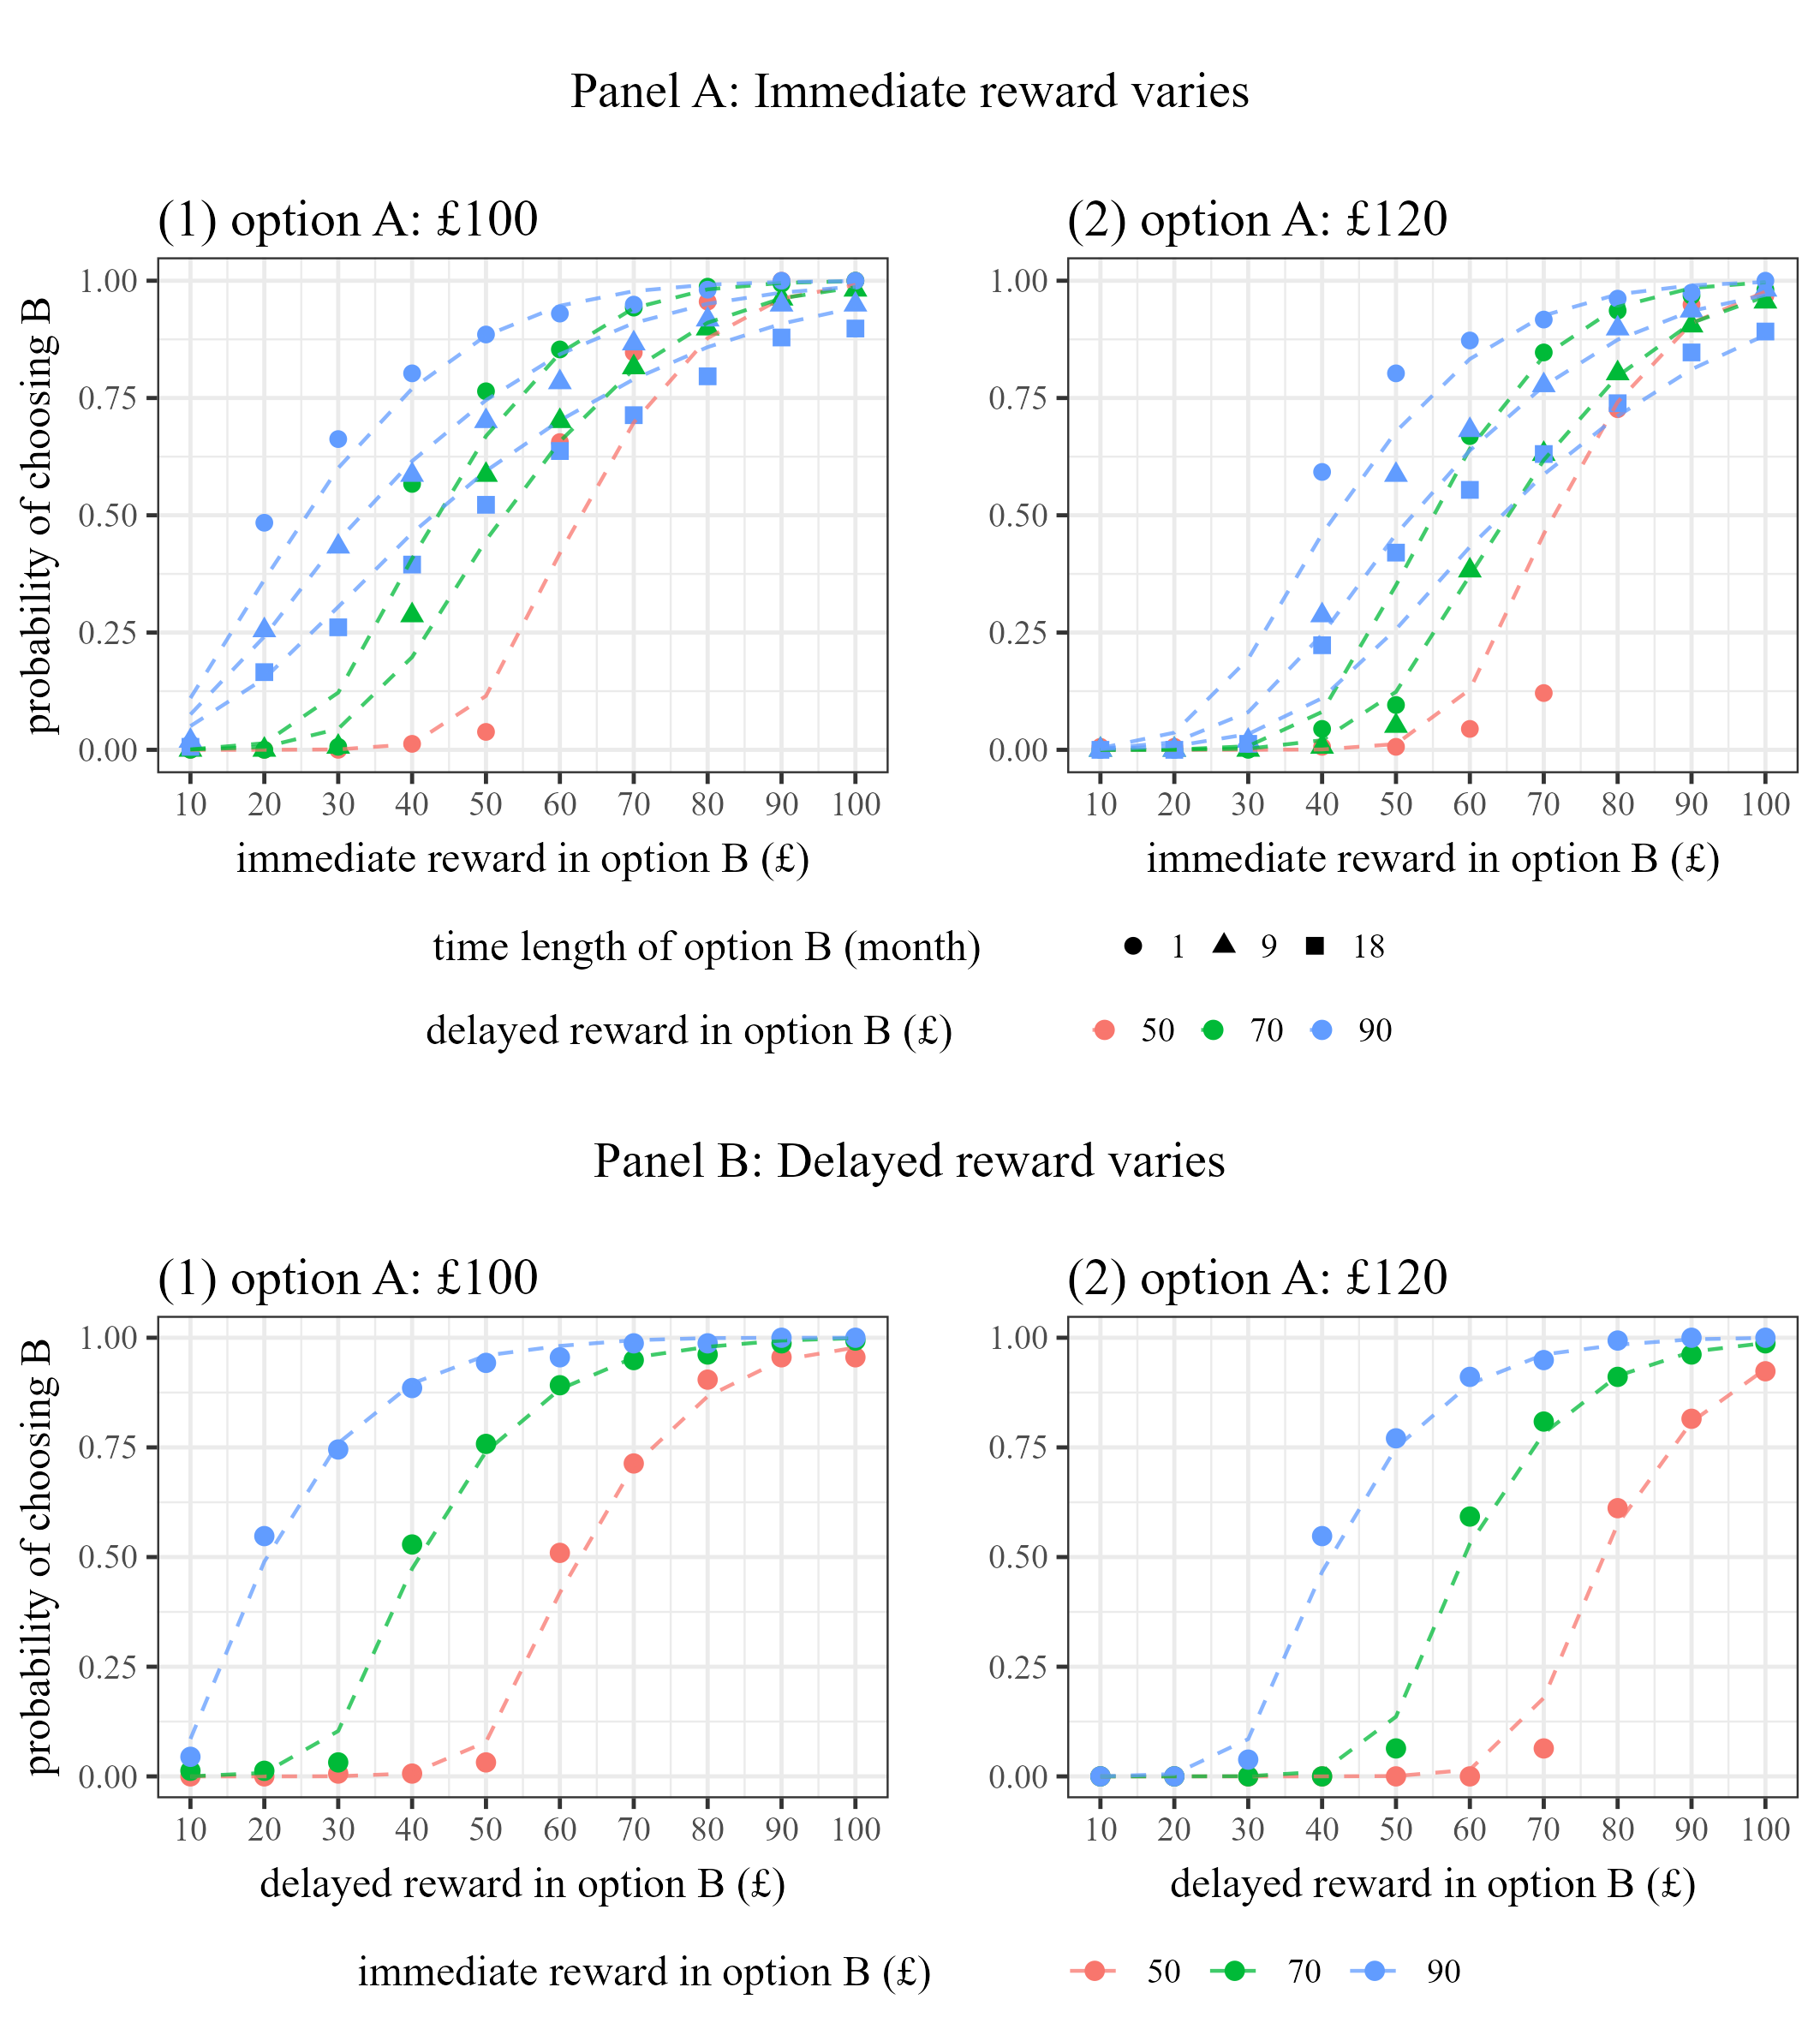
\includegraphics[width=0.96\textwidth]{figures/fig_grand_pred.png}
  \caption{Data and model predicted choice probabilities.}
  \caption*{\footnotesize Dots are the propotions of participants choosing the sequence option in the data, dashed curves are the mean predicted choice probabilities for sequence option. The curves are fitted by Model (5), a logit model on the censored data, with $X_v$ being transformed to $u(X_v)$, $M$ being added into interaction terms.}
  \label{fig:choice-predicted}
\end{figure}

\hypertarget{alternative-mechanisms}{%
\section{Alternative Mechanisms}\label{alternative-mechanisms}}

\renewcommand\refname{Reference}
  \bibliography{experiment-ref.bib}

\end{document}
